\chapter{Capítulo de Testes}\label{cap4}

Este capítulo apresenta diversos testes em \LaTeX.
Deverá ser removido ao final (Anderson).

\section{Citações}

Teste de Citação direta com mais de 3 linhas:

\begin{citacao}
As citações diretas, no texto, com mais de três linhas, devem ser
destacadas com recuo de 4 cm da margem esquerda, com letra menor que a do texto
utilizado e sem as aspas. No caso de documentos datilografados, deve-se
observar apenas o recuo \cite[5.3]{NBR10520:2002}.
\end{citacao}


Outras citações:

É amplamente sabido e divulgado que esta linha encontra-se neste local apenas para ocupar espaço \cite{van86}.

De forma análoga, \citeonline{macedo2005} diz que ``Batatinha quando nasce se esparrama pelo chão, menininha quando dorme, põe a mão no coração''. 

Note que em \LaTeX, as aspas iniciais e finais \emph{no código} são diferentes, mas no texto compilado elas se apresentam como aspas inglesas.



\section{Figuras}


\begin{figure}[h]
	\caption{\label{fig_app}Aplicativo A}
	\begin{center}
	    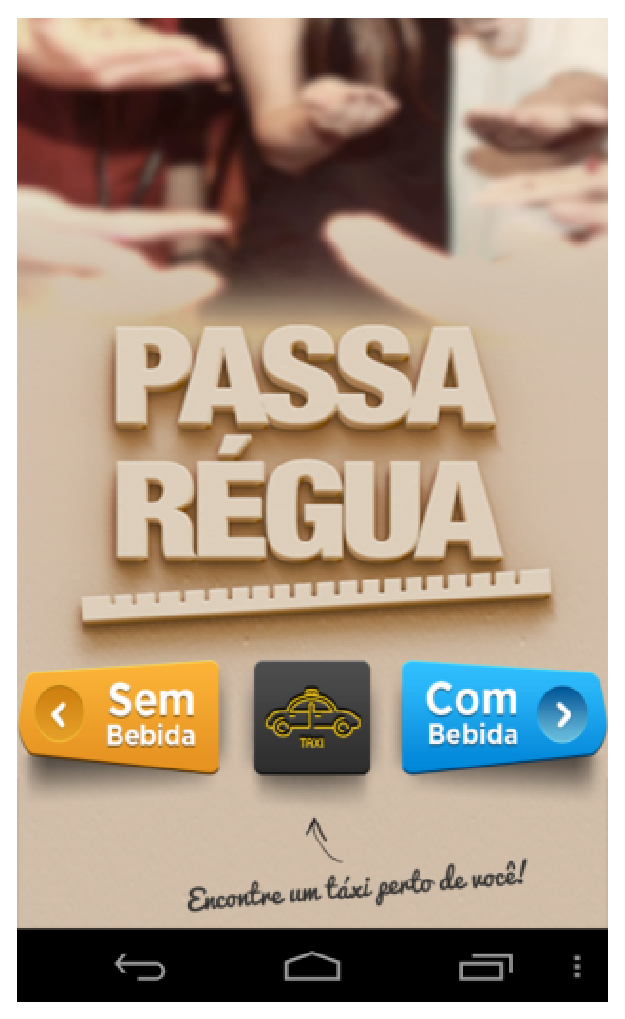
\includegraphics[scale=0.3]{image1}
	\end{center}
	\legend{Fonte: \citeonline[p. 24]{araujo2012}}
\end{figure}



% ---
\section{Expressões matemáticas}
% ---

\index{expressões matemáticas}Use o ambiente \texttt{equation} para escrever
expressões matemáticas numeradas:

\begin{equation}
  \forall x \in X, \quad \exists \: y \leq \epsilon
\end{equation}

Escreva expressões matemáticas entre \$ e \$, como em $ \lim_{x \to \infty}
\exp(-x) = 0 $, para que fiquem na mesma linha.

